\documentclass{article}
\usepackage[utf8]{inputenc} % Required for inputting international characters
\usepackage[T1]{fontenc} % Output font encoding for international characters

%%%%%%%%%%%%%%%%%%%%%%%%%%%%%%%%%
% PACKAGE IMPORTS
%%%%%%%%%%%%%%%%%%%%%%%%%%%%%%%%%
\usepackage[tmargin=2cm,rmargin=1in,lmargin=1in,margin=0.85in,bmargin=2cm,footskip=.2in]{geometry}
\usepackage{amsmath,amsfonts,amsthm,amssymb,mathtools} %general maths stuff
\usepackage[varbb]{newpxmath} %maths tools
\usepackage{xfrac} %a/b fractions
\usepackage[makeroom]{cancel}
\usepackage{mathtools}
\usepackage{bookmark}
\usepackage{enumitem}
\usepackage{hyperref,theoremref}
\hypersetup{
	pdftitle={Past Paper},
	colorlinks=true, linkcolor=black!90,
	bookmarksnumbered=true,
	bookmarksopen=true
}
\usepackage[most,many,breakable]{tcolorbox}
\usepackage{xcolor}
\usepackage{varwidth}
\usepackage{varwidth}
\usepackage{etoolbox}
\usepackage{nameref}
\usepackage{multicol,array}
\usepackage{tikz-cd}
\usepackage[ruled,vlined,linesnumbered]{algorithm2e}
\usepackage{comment} % enables the use of multi-line comments (\ifx \fi) 
\usepackage{import}
\usepackage{xifthen}
\usepackage{pdfpages}
\usepackage{transparent}
\usepackage{tikzsymbols}

\usepackage[default]{raleway}
\usepackage{sectsty}
\renewcommand*\familydefault{\sfdefault} % Force the sans-serif version of any font used
\allsectionsfont{\sffamily\mdseries\upshape} % (See the fntguide.pdf for font help)

\usepackage[nottoc,notlof,notlot]{tocbibind} % Put the bibliography in the ToC
\usepackage[titles,subfigure]{tocloft} % Alter the style of the Table of Contents
\renewcommand{\cftsecfont}{\rmfamily\mdseries\upshape}
\renewcommand{\cftsecpagefont}{\rmfamily\mdseries\upshape} % No bold!

\usepackage{calc}
\usepackage{subfig}
\usepackage{pgfplots}
\pgfplotsset{compat = newest}


%%%%%%%%%%%%%%%%%%%%%%%%%%%%%%J
% SELF MADE COLORS
%%%%%%%%%%%%%%%%%%%%%%%%%%%%%%

\definecolor{myg}{RGB}{56, 140, 70}
\definecolor{myb}{RGB}{45, 111, 177}
\definecolor{myr}{RGB}{199, 68, 64}
\definecolor{mytheorembg}{HTML}{F2F2F9}
\definecolor{mytheoremfr}{HTML}{00007B}
\definecolor{mylenmabg}{HTML}{FFFAF8}
\definecolor{mylenmafr}{HTML}{983b0f}
\definecolor{mypropbg}{HTML}{f2fbfc}
\definecolor{mypropfr}{HTML}{191971}
\definecolor{myexamplebg}{HTML}{F2FBF8}
\definecolor{myexamplefr}{HTML}{88D6D1}
\definecolor{myexampleti}{HTML}{2A7F7F}
\definecolor{mydefinitbg}{HTML}{E5E5FF}
\definecolor{mydefinitfr}{HTML}{3F3FA3}
\definecolor{notesgreen}{RGB}{0,162,0}
\definecolor{myp}{RGB}{197, 92, 212}
\definecolor{mygr}{HTML}{2C3338}
\definecolor{myred}{RGB}{127,0,0}
\definecolor{myyellow}{RGB}{169,121,69}
\definecolor{myexercisebg}{HTML}{F2FBF8}
\definecolor{myexercisefg}{HTML}{88D6D1}


%%%%%%%%%%%%%%%%%%%%%%%%%%%%
% TCOLORBOX SETUPS
%%%%%%%%%%%%%%%%%%%%%%%%%%%%
%================================
% EXAMPLE BOX
%================================

\newtcbtheorem[number within=section]{Example}{Example}
{%
	colback = myexamplebg
	,breakable
	,colframe = myexamplefr
	,coltitle = myexampleti
	,boxrule = 1pt
	,sharp corners
	,detach title
	,before upper=\tcbtitle\par\smallskip
	,fonttitle = \bfseries
	,description font = \mdseries
	,separator sign none
	,description delimiters parenthesis
}
{ex}

%================================
% Question BOX
%================================

\makeatletter
\newtcbtheorem{question}{Question}{enhanced,
	breakable,
	colback=gray!20!white,
	colframe=mygr,
	attach boxed title to top left={yshift*=-\tcboxedtitleheight},
	fonttitle=\bfseries,
	title={#2},
	boxed title size=title,
	boxed title style={%
		sharp corners,
		rounded corners=northwest,
		colback=tcbcolframe,
		boxrule=0pt,
	},
	underlay boxed title={%
		\path[fill=tcbcolframe] (title.south west)--(title.south east)
		to[out=0, in=180] ([xshift=5mm]title.east)--
		(title.center-|frame.east)
		[rounded corners=\kvtcb@arc] |-
		(frame.north) -| cycle;
	},
	#1
}{def}
\makeatother


%================================
% NOTE BOX
%================================


\usetikzlibrary{arrows,calc,shadows.blur}
\tcbuselibrary{skins}
\newtcolorbox{questionpart}[2][]{%
	enhanced jigsaw,
	colback=white,
	colframe=gray!80!black,
	size=small,
	boxrule=1pt,
	title=\textit{#2},
	halign title=flush center,
	coltitle=black,
	breakable,
	drop shadow=black!50!white,
	attach boxed title to top left={xshift=0.2cm,yshift=-\tcboxedtitleheight/2,yshifttext=-\tcboxedtitleheight/2},
	minipage boxed title=0.5cm,
	boxed title style={%
		colback=white,
		size=fbox,
		boxrule=1pt,
		boxsep=2pt,
		underlay={%
			\coordinate (dotA) at ($(interior.west) + (-0.5pt,0)$);
			\coordinate (dotB) at ($(interior.east) + (0.5pt,0)$);
			\begin{scope}
				\clip (interior.north west) rectangle ([xshift=3ex]interior.east);
				\filldraw [white, blur shadow={shadow opacity=60, shadow yshift=-.75ex}, rounded corners=2pt] (interior.north west) rectangle (interior.south east);
			\end{scope}
			\begin{scope}[gray!80!black]
				\fill (dotA) circle (2pt);
				\fill (dotB) circle (2pt);
			\end{scope}
		},
	},
	#1,
}

%%%%%%%%%%%%%%%%%%%%%%%%%%%%%%
% SELF MADE COMMANDS
%%%%%%%%%%%%%%%%%%%%%%%%%%%%%%

\newcommand{\qs}[1]{\begin{question}{}{}#1\end{question}}
\newcommand{\qsp}[2]{\begin{questionpart}{#1}{}#2\end{questionpart}}

\newcommand{\plotbasic}[3][black]{ % colour func formatted
		\begin{tikzpicture}
		\begin{axis}[
				axis lines = center,
				xlabel = \(x\),
				ylabel = \(f(x)\),
			]
			
			\addplot [
				domain=-5:5, 
				samples=100, 
				color={#1},
			]
			{#2};
			\addlegendentry{#3}
		\end{axis}
	\end{tikzpicture}
}
\newenvironment{plotter}{
	\begin{tikzpicture}
		\begin{axis}[
			axis lines = center,
			xlabel = \(x\),
			ylabel = \(f(x)\),
		]
}
{
\end{axis}
\end{tikzpicture}
}


\newenvironment{unitcircled}{
\usetikzlibrary {intersections}
\begin{tikzpicture}[scale=2]
	\draw[step=.5cm,gray,very thin] (-1.2,-1.2) grid (1.2,1.2);
	\draw[->] (-1.2,0) -- (1.2,0) coordinate (x axis);
	\draw[->] (0,-1.2) -- (0,1.2) coordinate (y axis);
	\draw (0,0) circle [radius=1cm];
	
	\foreach \x/\xtext in {-1, -0.5/-\frac{1}{2}, 0, 0.5/\frac{1}{2}, 1}
	\draw (\x cm,1pt) -- (\x cm,-1pt) node[anchor=north,fill=white] {$\xtext$};
	\foreach \y/\ytext in {-1, -0.5/-\frac{1}{2}, 0.5/\frac{1}{2}, 1}
	\draw (1pt,\y cm) -- (-1pt,\y cm) node[anchor=east,fill=white] {$\ytext$};
} {
\end{tikzpicture}
}

\newcommand*\circled[1]{\tikz[baseline=(char.base)]{
	\node[shape=circle,draw,inner sep=1pt] (char) {#1};}}
\newcommand\getcurrentref[1]{%
\ifnumequal{\value{#1}}{0}
{??}
{\the\value{#1}}%
}
\newcommand{\getCurrentSectionNumber}{\getcurrentref{section}}


\newcounter{mylabelcounter}

\makeatletter
\newcommand{\setword}[2]{%
\phantomsection
#1\def\@currentlabel{\unexpanded{#1}}\label{#2}%
}
\makeatother

\tikzset{
symbol/.style={
	draw=none,
	every to/.append style={
		edge node={node [sloped, allow upside down, auto=false]{$#1$}}}
}
}


%%%%%%%%%%%%%%%%%%%%%%%%%%%%%%%%%%%%%%%%%%%
% TABLE OF CONTENTS
%%%%%%%%%%%%%%%%%%%%%%%%%%%%%%%%%%%%%%%%%%%

\usepackage{tikz}
\definecolor{doc}{RGB}{0,60,110}
\usepackage{titletoc}
\contentsmargin{0cm}
\titlecontents{chapter}[3.7pc]
{\addvspace{30pt}%
	\begin{tikzpicture}[remember picture, overlay]%
		\draw[fill=doc!60,draw=doc!60] (-7,-.1) rectangle (-0.9,.5);%
		\pgftext[left,x=-3.5cm,y=0.2cm]{\color{white}\Large\sc\bfseries Chapter\ \thecontentslabel};%
	\end{tikzpicture}\color{doc!60}\large\sc\bfseries}%
{}
{}
{\;\titlerule\;\large\sc\bfseries Page \thecontentspage
	\begin{tikzpicture}[remember picture, overlay]
		\draw[fill=doc!60,draw=doc!60] (2pt,0) rectangle (4,0.1pt);
\end{tikzpicture}}%
\titlecontents{section}[3.7pc]
{\addvspace{2pt}}
{\contentslabel[\thecontentslabel]{2pc}}
{}
{\hfill\small \thecontentspage}
[]
\titlecontents*{subsection}[3.7pc]
{\addvspace{-1pt}\small}
{}
{}
{\ --- \small\thecontentspage}
[ \textbullet\ ][]

\makeatletter
\renewcommand{\tableofcontents}{%
	\chapter*{%
		\vspace*{-20\p@}%
		\begin{tikzpicture}[remember picture, overlay]%
			\pgftext[right,x=15cm,y=0.2cm]{\color{doc!60}\Huge\sc\bfseries \contentsname};%
			\draw[fill=doc!60,draw=doc!60] (13,-.75) rectangle (20,1);%
			\clip (13,-.75) rectangle (20,1);
			\pgftext[right,x=15cm,y=0.2cm]{\color{white}\Huge\sc\bfseries \contentsname};%
	\end{tikzpicture}}%
	\@starttoc{toc}}
\makeatother
%Symbols
\newcommand{\dg}{^\circ}
\newcommand{\dang}{\measuredangle} %% Directed angle
\newcommand{\lm}{\lambda}
\newcommand{\uin}{\mathbin{\rotatebox[origin=c]{90}{$\in$}}}
\newcommand{\usubset}{\mathbin{\rotatebox[origin=c]{90}{$\subset$}}}

%Shortcuts
\newcommand{\ii}{\item}
\newcommand{\lthen}{\rightarrow}
\newcommand{\opname}{\operatorname}

%Diff/Int
\newcommand{\differen}[1][y]{\frac{\Delta #1}{\Delta x}}
\newcommand{\differend}[1][y]{\dfrac{\Delta #1}{\Delta x}}
\newcommand{\twodifferen}[1][y]{\frac{\Delta^2 #1}{\Delta x^2}}
\newcommand{\twodifferend}[1][y]{\dfrac{\Delta^2 #1}{\Delta x^2}}
\newcommand{\limit}[2]{\lim\limits_{#1 \to #2}}
\newcommand{\integratestart}[4][x]{\int_{#3}^{#4} \left( {#2} \right) d{#1}} %x/t/etc func lowerlim upperlim
\newcommand{\integrateinner}[3]{\left[ {#1} \right]_{#2}^{#3}} % func lowerlim upperlim

\DeclareMathOperator{\cosec}{cosec}
\DeclareMathOperator{\ud}{\textit{undefined}}

\newcommand{\func}[2][f]{#1 \left( #2 \right)}


%---------------------------------------
% BlackBoard Math Fonts :-
%---------------------------------------

%Captital Letters
\newcommand{\bbA}{\mathbb{A}}	\newcommand{\bbB}{\mathbb{B}}
\newcommand{\bbC}{\mathbb{C}}	\newcommand{\bbD}{\mathbb{D}}
\newcommand{\bbE}{\mathbb{E}}	\newcommand{\bbF}{\mathbb{F}}
\newcommand{\bbG}{\mathbb{G}}	\newcommand{\bbH}{\mathbb{H}}
\newcommand{\bbI}{\mathbb{I}}	\newcommand{\bbJ}{\mathbb{J}}
\newcommand{\bbK}{\mathbb{K}}	\newcommand{\bbL}{\mathbb{L}}
\newcommand{\bbM}{\mathbb{M}}	\newcommand{\bbN}{\mathbb{N}}
\newcommand{\bbO}{\mathbb{O}}	\newcommand{\bbP}{\mathbb{P}}
\newcommand{\bbQ}{\mathbb{Q}}	\newcommand{\bbR}{\mathbb{R}}
\newcommand{\bbS}{\mathbb{S}}	\newcommand{\bbT}{\mathbb{T}}
\newcommand{\bbU}{\mathbb{U}}	\newcommand{\bbV}{\mathbb{V}}
\newcommand{\bbW}{\mathbb{W}}	\newcommand{\bbX}{\mathbb{X}}
\newcommand{\bbY}{\mathbb{Y}}	\newcommand{\bbZ}{\mathbb{Z}}

%---------------------------------------
% MathCal Fonts :-
%---------------------------------------

%Captital Letters
\newcommand{\mcA}{\mathcal{A}}	\newcommand{\mcB}{\mathcal{B}}
\newcommand{\mcC}{\mathcal{C}}	\newcommand{\mcD}{\mathcal{D}}
\newcommand{\mcE}{\mathcal{E}}	\newcommand{\mcF}{\mathcal{F}}
\newcommand{\mcG}{\mathcal{G}}	\newcommand{\mcH}{\mathcal{H}}
\newcommand{\mcI}{\mathcal{I}}	\newcommand{\mcJ}{\mathcal{J}}
\newcommand{\mcK}{\mathcal{K}}	\newcommand{\mcL}{\mathcal{L}}
\newcommand{\mcM}{\mathcal{M}}	\newcommand{\mcN}{\mathcal{N}}
\newcommand{\mcO}{\mathcal{O}}	\newcommand{\mcP}{\mathcal{P}}
\newcommand{\mcQ}{\mathcal{Q}}	\newcommand{\mcR}{\mathcal{R}}
\newcommand{\mcS}{\mathcal{S}}	\newcommand{\mcT}{\mathcal{T}}
\newcommand{\mcU}{\mathcal{U}}	\newcommand{\mcV}{\mathcal{V}}
\newcommand{\mcW}{\mathcal{W}}	\newcommand{\mcX}{\mathcal{X}}
\newcommand{\mcY}{\mathcal{Y}}	\newcommand{\mcZ}{\mathcal{Z}}


%---------------------------------------
% Bold Math Fonts :-
%---------------------------------------

%Captital Letters
\newcommand{\bmA}{\boldsymbol{A}}	\newcommand{\bmB}{\boldsymbol{B}}
\newcommand{\bmC}{\boldsymbol{C}}	\newcommand{\bmD}{\boldsymbol{D}}
\newcommand{\bmE}{\boldsymbol{E}}	\newcommand{\bmF}{\boldsymbol{F}}
\newcommand{\bmG}{\boldsymbol{G}}	\newcommand{\bmH}{\boldsymbol{H}}
\newcommand{\bmI}{\boldsymbol{I}}	\newcommand{\bmJ}{\boldsymbol{J}}
\newcommand{\bmK}{\boldsymbol{K}}	\newcommand{\bmL}{\boldsymbol{L}}
\newcommand{\bmM}{\boldsymbol{M}}	\newcommand{\bmN}{\boldsymbol{N}}
\newcommand{\bmO}{\boldsymbol{O}}	\newcommand{\bmP}{\boldsymbol{P}}
\newcommand{\bmQ}{\boldsymbol{Q}}	\newcommand{\bmR}{\boldsymbol{R}}
\newcommand{\bmS}{\boldsymbol{S}}	\newcommand{\bmT}{\boldsymbol{T}}
\newcommand{\bmU}{\boldsymbol{U}}	\newcommand{\bmV}{\boldsymbol{V}}
\newcommand{\bmW}{\boldsymbol{W}}	\newcommand{\bmX}{\boldsymbol{X}}
\newcommand{\bmY}{\boldsymbol{Y}}	\newcommand{\bmZ}{\boldsymbol{Z}}
%Small Letters
\newcommand{\bma}{\boldsymbol{a}}	\newcommand{\bmb}{\boldsymbol{b}}
\newcommand{\bmc}{\boldsymbol{c}}	\newcommand{\bmd}{\boldsymbol{d}}
\newcommand{\bme}{\boldsymbol{e}}	\newcommand{\bmf}{\boldsymbol{f}}
\newcommand{\bmg}{\boldsymbol{g}}	\newcommand{\bmh}{\boldsymbol{h}}
\newcommand{\bmi}{\boldsymbol{i}}	\newcommand{\bmj}{\boldsymbol{j}}
\newcommand{\bmk}{\boldsymbol{k}}	\newcommand{\bml}{\boldsymbol{l}}
\newcommand{\bmm}{\boldsymbol{m}}	\newcommand{\bmn}{\boldsymbol{n}}
\newcommand{\bmo}{\boldsymbol{o}}	\newcommand{\bmp}{\boldsymbol{p}}
\newcommand{\bmq}{\boldsymbol{q}}	\newcommand{\bmr}{\boldsymbol{r}}
\newcommand{\bms}{\boldsymbol{s}}	\newcommand{\bmt}{\boldsymbol{t}}
\newcommand{\bmu}{\boldsymbol{u}}	\newcommand{\bmv}{\boldsymbol{v}}
\newcommand{\bmw}{\boldsymbol{w}}	\newcommand{\bmx}{\boldsymbol{x}}
\newcommand{\bmy}{\boldsymbol{y}}	\newcommand{\bmz}{\boldsymbol{z}}

\graphicspath{{./images/}}

\title{\huge{C3 Z}}
\author{\huge{Jack Maguire}}
\date{}

\begin{document}
\maketitle

\qs{
\begin{align*}
	x &= \ln \left( y^2 + 9 \right)^\frac{3}{2} \\
	  &= \left( \ln \left( y^2 + 9 \right) \right) ^\frac{3}{2} \\
	u &= \ln \left( y^2 + 9 \right) \\
	\frac{\Delta u}{\Delta x} &= \frac{2y}{y^2 + 9} \\
	\frac{\Delta y}{\Delta x} &= \frac{3}{2} \left( \ln \left( y^2 + 9 \right) \right) ^ \frac{1}{2} \frac{2y}{y^2 + 9} \\
	&= \frac{6y}{2y^2 + 18} \sqrt{\ln \left( y^2 + 9 \right)} \\
\end{align*}
\text{Question wrong? Cannot get to simplify and desmos disagrees}
}
\qs{
\begin{align*}
	\frac{\sin 2 \phi}{\sin \phi} - \frac{\cos 2 \phi}{\cos \phi} &\equiv \sec \phi \\
	\textbf{LHS} &\equiv \frac{\sin 2 \phi}{\sin \phi} - \frac{\cos 2 \phi}{\cos \phi} \\
	&\equiv \frac{2 \sin  \cos \phi}{\sin \phi} - \frac{2\cos^2 \phi - 1}{\cos \phi} \\
	&\equiv 2 \cos \phi - 2\cos \phi + \sec \phi \equiv \sec \phi \equiv \textbf{RHS} \qed
\end{align*}
}

\qs{
\qsp{a}{
	\begin{multicols}{2}
		\noindent
		\begin{align*}
			v &=  1 + 2 \ln x \\
			v^\prime &= \frac{2}{x}
		\end{align*}
		\columnbreak
		\begin{align*}
			u &= x \\
			u^\prime &= 1
		\end{align*}
	\end{multicols}
	\begin{align*}
		\differen &= \frac{vu^\prime  - v^\prime u}{v^2} \\
		&= \frac{1 + 2 \ln x - \frac{2x}{x}}{(1 + 2 \ln x)^2} \\
		&= \frac{2 \ln x - 1}{1 + 4 \ln x + 4 (\ln x)^2} \\
		0 &= \frac{2 \ln x - 1}{1 + 4 \ln x + 4 (\ln x)^2} \\
		0 &= 2 \ln x - 1 \\
		\frac{1}{2} &= \ln x \\
		x &= e^\frac{1}{2} = \sqrt{e} \\
		y &= \frac{x}{1 + 2 \ln x} \\
		  &= \frac{\sqrt{e}}{1 + 1} \\
		  &= \frac{1}{2}\sqrt{e} \\
		\text{TP} &= (\sqrt{e}, \frac{1}{2}\sqrt{e})
	\end{align*}
}
\qsp{b}{
	\begin{multicols}{2}
		\noindent
		\begin{align*}
			v &= (1 + 2 \ln x)^2 \\
			v^\prime &= \frac{4 + 8 \ln x}{x}
		\end{align*}
		\columnbreak
		\begin{align*}
			u &= 2\ln x - 1 \\
			u^\prime &= \frac{2}{x}
		\end{align*}
	\end{multicols}
	\begin{align*}
		\differen &= \frac{vu^\prime  - v^\prime u}{v^2} \\
		\twodifferen &= \frac{\frac{2}{x}(1 + 2 \ln x)^2 - \frac{4 + 8 \ln x}{x}(2\ln x - 1)}{(1 + 2 \ln x)^4} \\
		\twodifferen_{\sqrt{e}} &= \frac{\frac{2}{\sqrt{e}}(1 + 1)^2 - \frac{4 +4}{\sqrt{e}}(1 - 1)}{(1 + 1)^4} \\
		&= \frac{\frac{2}{\sqrt{e}}}{(1 + 1)^2} \\
		&= \frac{2}{4\sqrt{e}} \\
		&= \frac{1}{2\sqrt{e}} 
	\end{align*}
	\( \frac{1}{2\sqrt{e}} > 0 \therefore \) is a minimum point.
}
}

\qs{
\qsp{a}{
	\begin{align*}
		x &= \tan y \\
		\frac{\Delta x}{\Delta y} &= \sec^2 y \\
		\frac{\Delta y}{\Delta x} &= \cos^2 y \\
		&= \cos^2 \left( \tan^{-1} x \right) \\
		\textbf{???}
	\end{align*}
}
\qsp{b}{
	\begin{align*}
		\differen &= 1 + x^2 - \frac{8}{1+x^2} - 6x \\
		&= x^2 - 6x - \frac{8}{1+x^2} + 1 \\
		0 &= x^2 - 6x - \frac{8}{1+x^2} + 1 \\
		&= \left( 1 + x^2 \right)x^2 - \left( 1 + x^2 \right)6x - 8 + \left( 1 + x^2 \right) \\
		&= x^2 + x^4 - 6x - 6x^3 -8 + 1 + x^2 \\
		&= x^4 - 6x^3 + 2x^2 -6x - 7 \\
		& \textbf{???}
	\end{align*}
}
\qsp{c}{
	\begin{align*}
		\func{x} &= 6x^3+14x-1
		\func{0} &= -1 \\
		\func{1} &= 19 \\
	\end{align*}
	Between positive and negative \( \therefore \) root inbetween.
}
\qsp{d}{
	\textbf{???}
}
\qsp{e}{
	\textbf{???}
}
}

\qs{
\qsp{a}{
	\begin{align*}
		H &= k \left( 1 - e^{-\frac{1}{12}t} \right) \\
		41 &= k \left( 1 - e^{-\frac{5}{12}} \right) \\
		\frac{41}{k} &= 1 - e^{-\frac{5}{12}} \\
		k &= \frac{41}{1 - e^{-\frac{5}{12}}} \\
		k &= 120.319 \ldots \\
		&= 120
	\end{align*}
}
\qsp{b}{
	\begin{align*}
		H &= 120 \left( 1 - e^{-\frac{1}{12}t} \right) \\
		\frac{90}{120} &= 1 - e^{-\frac{1}{12}t} \\
		\frac{1}{4} &= e^{-\frac{1}{12}t} \\
		\ln \frac{1}{4} &= -\frac{1}{12} t \\
		-12t &= - \ln 4 \\
		t &= 12 \ln 4 \\
		&= 24 \ln 2
	\end{align*}
}
\qsp{c}{
	\begin{align*}
		H &= 120 \left( 1 - e^{-\frac{1}{12}t} \right) \\
		\frac{H}{120} &= 1 - e^{-\frac{1}{12}t} \\
		1 - \frac{H}{120} &= e^{-\frac{1}{12}t} \\
		-\frac{1}{12}t &= \ln \left( 1 - \frac{H}{120} \right) \\
		t &= -12 \ln \left( 1 - \frac{H}{120} \right) \\
		\\
		H &= 120 \left( 1 - e^{-\frac{1}{12}t} \right) \\
		a &= 1 - e^{-\frac{1}{12}t} \\
		\frac{\Delta a}{\Delta t} &= \frac{1}{12} e^{-\frac{1}{12}t} \\
		\frac{\Delta H}{\Delta t} &= 120\frac{1}{12} e^{-\frac{1}{12}t} \\
		&= 10 e^{-\frac{1}{12}t} \\
		&= 10e^{-12 \ln \left( 1 - \frac{H}{120} \right)} \\
		&= \frac{-10}{12} H
	\end{align*}
}
\qsp{d}{
	\begin{align*}
		\frac{\Delta H}{\Delta t} &= \frac{-10}{12} H
		\frac{\Delta H}{\Delta t}_7.5 &= -\frac{-10}{12}7.5 \\
		&= \frac{-25}{4} \\
	\end{align*}
}
\qsp{e}{
	\begin{align*}
		\frac{\Delta H}{\Delta t} &= 120\frac{1}{12} e^{-\frac{1}{12}t} \\
		0 &= 10 e^{-\frac{1}{12}t} \\
		e^{-\frac{1}{12}t} &= 0 \\
	\end{align*}
	Since \(\bbR \nsubseteq \ln 0\), we can see that this model exponentially grows, that is, there is no maximum height.
}
}

\qs{
\qsp{a}{
	\[ 	2 \leq \func{x} \leq 4 \]
	\[ a = 3 \]
	\[ \pi \to 2 \pi \therefore b = 0.5 \]
}
\qsp{b}{
	\begin{align*}
		y &= 3 + \cos \frac{x}{2} \\
		x &= 3 + \cos \frac{y}{2} \\
		\cos \frac{y}{2} &= x - 3\\
		y &= 2 \cos^{-1} ( x - 3 ) \\
	\end{align*}
}
\qsp{c}{
	\[ 2 \leq x \leq 4 \]
	\[ 0 \leq \func{x} \leq 2 \pi \]
}
\qsp{d}{
	\begin{align*}
		\differen &= -\frac{1}{2} \sin \frac{x}{2}
		\differen_{\frac{4}{3}\pi} &= -\frac{1}{2} \sin \frac{2\pi}{3} \\
		&= -\frac{1}{2} \frac{\sqrt{3}}{2} \\
		&= -\frac{\sqrt{3}}{4} 
	\end{align*}
}
\qsp{e}{
\[ -\frac{\sqrt{3}}{4}  \]
}
}

\qs{
\qsp{a}{
	\begin{align*}
		\sin P + \sin Q  &\equiv 2 \sin \left( \frac{P+Q}{2} \right) \cos \left( \frac{P-Q}{2} \right) \\
		\textbf{RHS} &\equiv 2 \sin \left( \frac{P+Q}{2} \right) \cos \left( \frac{P-Q}{2} \right) \\
		&\equiv 2 \sin \left( \frac{P}{2} + \frac{Q}{2} \right) \cos \left( \frac{P}{2} - \frac{Q}{2} \right) \\
		&\equiv 2 \left( \sin \frac{P}{2} \cos \frac{Q}{2} + \sin \frac{Q}{2} \cos \frac{P}{2} \right) \left( \cos \frac{P}{2} \cos \frac{Q}{2} + \sin \frac{P}{2} \sin \frac{Q}{2}  \right) \\
		&\equiv 2 \left( \sin \frac{P}{2} \cos \frac{P}{2} \cos^2 \frac{Q}{2} + \sin^2 \frac{P}{2} \sin \frac{Q}{2} \cos \frac{Q}{2} + \sin \frac{Q}{2} \cos^2 \frac{P}{2} \cos \frac{Q}{2} + \sin \frac{P}{2} \sin^2 \frac{Q}{2} \cos \frac{P}{2} \right) \\
		& \textbf{???} \\
		&\equiv \sin P + \sin Q \equiv \text{RHS} \qed
	\end{align*}
}
\qsp{b}{
	\begin{align*}
		\sin \theta - \sin 3 \theta + \sin 5 \theta &= 0 
		\textbf{???}
	\end{align*}
}
}

\qs{
	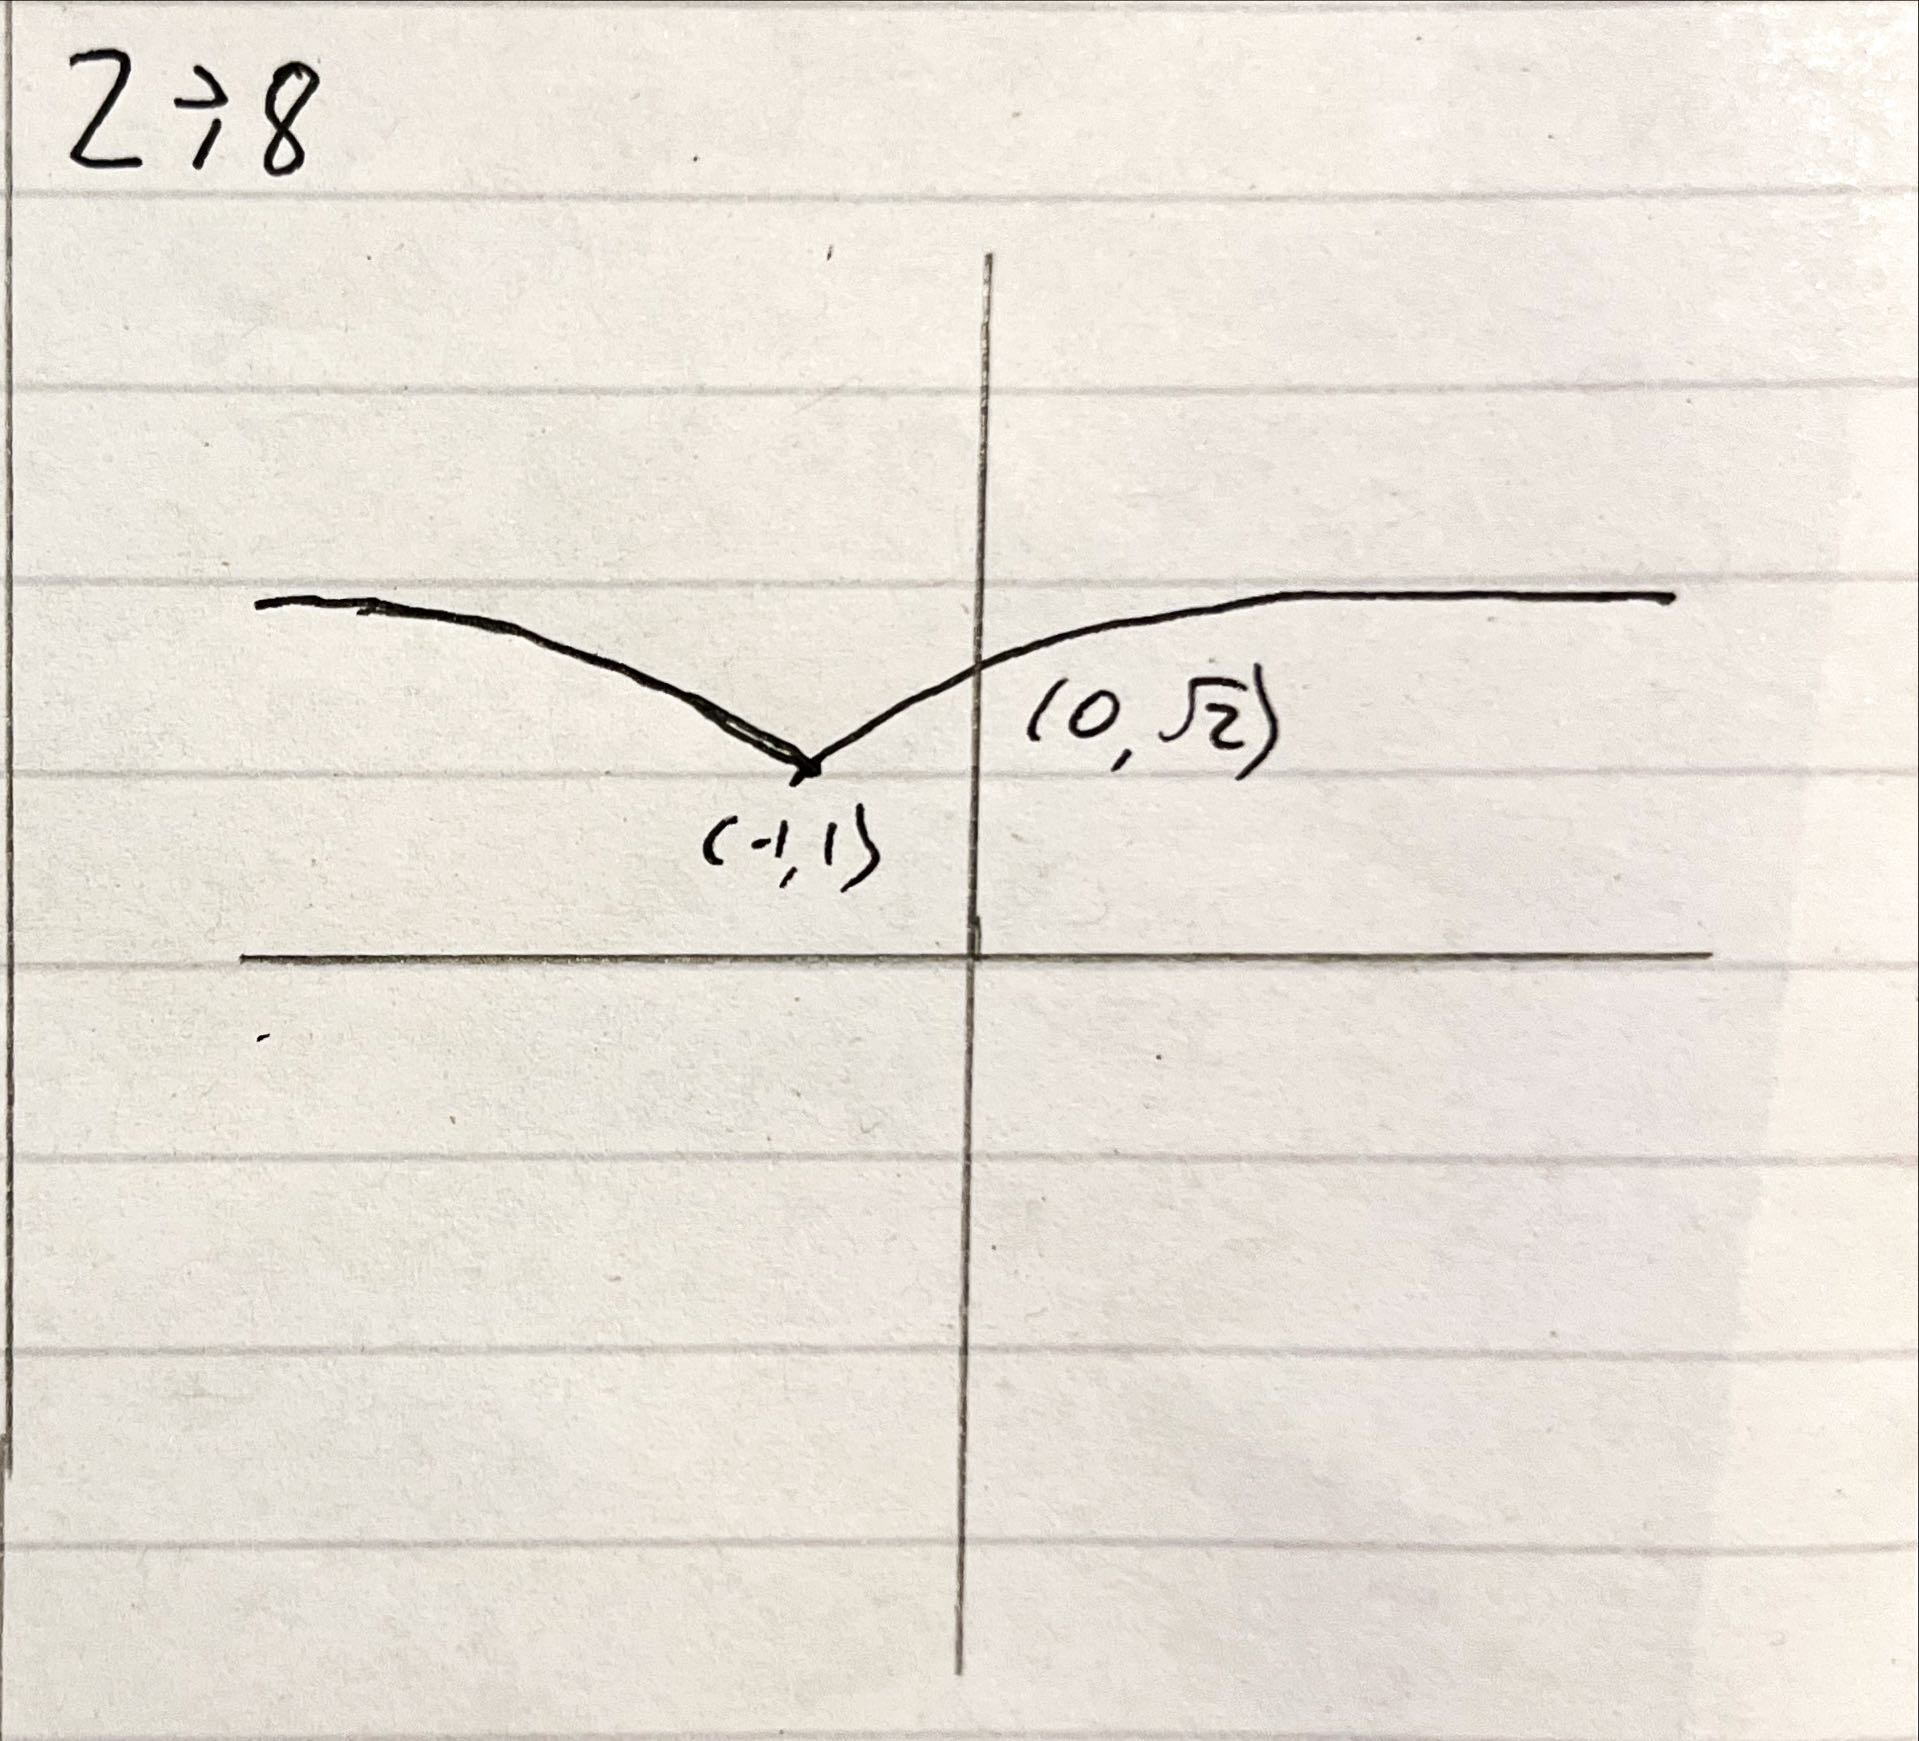
\includegraphics[width=\textwidth / 3]{z8}
}
	
\end{document}